% !TEX root = ../main.tex
\subsection{Study Results}
\label{14.30::study_results}
    % Explain binning scheme selected.
    To select a region in $v_z$ to place the RG-E target, two criteria were considered: a phase space study and a statistics study.
    In the phase space study, the RG-F target gas region ($-30 < v_z < 20$ cm) was divided into ten 5 cm bins, and the phase space of each kinematic variable was analysed in each bin.
    The results of this study are presented in Section \ref{14.31::phase_space_study}.
    For the statistics study, the region chosen in the phase space study was further divided into 1 cm bins.
    The study aimed to determine which 7 cm region within the chosen range had the largest statistics.
    The validity of this choice was evaluated using a gemc simulation of the RG-E target system.
    The results of this study are presented in Section \ref{14.32::statistics_study}.

    % Statistical error estimation.
    Regarding the statistical error estimation, the total statistical error on the acceptance-corrected result, denoted as $e_\text{corr}$, needs to consider both the statistical error of the measurements ($e_\text{meas}$) and the acceptance correction ($e_\text{acc}$).
    The statistical error of the measurements, $e_\text{meas}$, is purely statistical in nature and is given by
    \begin{equation*}
        e_\text{meas} = \frac{\delta y_\text{meas}}{y_\text{meas}},
    \end{equation*}
    The acceptance correction error, $e_\text{acc}$, was derived in Equation \eqref{eq::14.20::acc_error}.

    Since $e_\text{meas}$ arises purely from experimental data and $e_\text{acc}$ is purely from simulation, they are considered to be completely uncorrelated.
    Therefore, the total statistical error of the acceptance-corrected result can be estimated as the quadratic addition of the two errors, i.e.,
    \begin{equation*}
        e_\text{corr} = \sqrt{e_\text{meas}^2 + e_\text{acc}^2}.
    \end{equation*}

    % !TEX root = ../main.tex
\subsubsection{Phase Space Study}
\label{14.31::phase_space_study}
    % Introduction.
    Considering the objectives of this DIS study, it is advantageous to maximise the phase space of each kinematic variable of study.
    This approach broadens the scope of investigation, increases sensitivity to detect rare phenomena, and facilitates the testing of theoretical predictions for future studies using the double target system.
    Therefore, the first criterion for selecting a $v_z$ region for the target is to find a region that provides the maximum range of kinematic variables.

    % Resulting plots.
    The resulting plots show the acceptance-corrected DIS variables separated into $v_z$ bins.
    Figures \ref{fig::14.31::q2_vz} and \ref{fig::14.31::nu_vz} display the distributions of the electron variables $Q^2$ and $\nu$, respectively.
    The $z_h$ distributions for $e^-\pi^+$ and $e^-\pi^-$ can be observed in Figures \ref{fig::14.31::zh_211_vz} and \ref{fig::14.31::zh_-211_vz}, respectively.
    Figures \ref{fig::14.31::pt2_211_vz} and \ref{fig::14.31::pt2_-211_vz} show the distributions of $p_T^2$ for $e^-\pi^+$ and $e^-\pi^-$, respectively.
    Finally, Figures \ref{fig::14.31::phipq_211_vz} and \ref{fig::14.31::phipq_-211_vz} present the distributions of $\phi_{PQ}$ for $e^-\pi^+$ and $e^-\pi^-$, respectively.
    These plots provide insights into the dependence of each DIS variable on the $v_z$ coordinate.

    % Q2.
    In the study of $Q^2$, as shown in Figure \ref{fig::14.31::q2_vz}, the higher end of the variable's phase space is limited for $v_z < -5$ cm, with the effect becoming more pronounced as we move further upstream.
    This effect can be understood by considering the compounded effect of the $\theta$ efficiency for negative particles (as seen in Figure \ref{fig::14.21::theta_study_neg}) and the limited acceptance region of FMT (described by Equation \eqref{eq::12.42::fmt_geometry_cut} and illustrated in Figure \ref{eq::12.42::vz_vs_theta}).

    The higher end of $\theta$ becomes limited for lower $v_z$ values.
    Based on the objective of maximising the phase space of each variable, this suggests setting the minimum $v_z$ for the RG-E target near $-5$ cm.
    Additionally, it is noted that the variable exhibits an unusual shape for $10$ cm $< v_z < 20$ cm, likely due to the cut in low $\theta$ angles in that region, which is another consequence of the FMT acceptance region.

    % nu.
    In the study of $\nu$, as seen in Figure \ref{fig::14.31::nu_vz}, it was previously observed that $\nu$ has no direct correlation with the scattering angle $\theta_C$ (Section \ref{14.20::acceptance_correction_results}).
    Therefore, no significant effect on the phase space of $\nu$ is observed for $v_z < -5$ cm, unlike $Q^2$.
    However, a loss is observed in the lower end of the phase space for $v_z = 10$ cm and downstream.
    Based on this effect, it is reasonable to keep $v_z$ below approximately 10 cm to preserve the largest possible phase space of $\nu$.

    % zh.
    In the study of $z_h$, despite its lack of direct correlation with the electron's and pion's $\theta$, clear differences are observed across different $v_z$ bins, as shown in Figures \ref{fig::14.31::zh_211_vz} and \ref{fig::14.31::zh_-211_vz}.
    However, this can be explained by its inverse correlation with $\nu$ (as described in Equation \eqref{eq::10.32::zh}).
    Similar to $\nu$, the extreme phase space loss is primarily observed for $v_z > 10$ cm, and therefore, no additional severe restrictions on the $v_z$ region are imposed beyond those defined based on the studies of $Q^2$ and $\nu$.

    % pt2.
    In the study of $p_T^2$, as depicted in Figures \ref{fig::14.31::pt2_211_vz} and \ref{fig::14.31::pt2_-211_vz}, large statistical fluctuations are observed for $p_T^2 > 1.4 \text{GeV}^2$, consistent with the prediction in Section \ref{14.22::hadronic_variables}.
    Studying the phase space of the variable, a cutoff at high $p_T^2$ values is observed for $v_z < -5$ cm and $v_z > 15$ cm, similar to what was seen for $Q^2$.
    Based on this observation, no additional restrictions are imposed on the $v_z$ region under study.

    % phipq.
    Regarding the study of $\phi_{PQ}$, as shown in Figures \ref{fig::14.31::phipq_211_vz} and \ref{fig::14.31::phipq_-211_vz}, no easily discernible loss is observed in the phase space of $\phi_{PQ}$ as we vary $v_z$.
    While there are significant changes in the shape of the variable distribution across different $v_z$ bins, conducting a detailed shape study is beyond the scope of this thesis, as ample information is already provided by the other DIS variables.

    % !TEX root = ../main.tex
\subsubsection{Statistics Study}
\label{14.32::statistics_study}
    After obtaining the $v_z$ region with the maximum range of kinematic variables, our second criterium is to maximise statistics inside this region.
    With phase space already maximised, this allows us to increase the statistical precision of future studies, enabling a thorough exploration of the parameter space.

    Based on the results of the different phase space studies, we'll limit the scope of this statistics study to the region $-5 \text{cm} < v_z < 10 \text{cm}$, the result of which can be observed in Figure \ref{fig::14.32::statistics}.
    The objective of this study is to find the 7 cm region in $v_z$ with the highest statistics.
    The choice of 7 cm in particular comes from the length of the double target, where the liquid target has a length of 3 cm, the separation between the liquid and solid target is of 4 cm, and the solid target is of negligible width for the scope of this study.

    First we look at $e^-$ statistics, seen in Figure \ref{fig::14.32::statistics_11}.
    It is trivial to note that, in the studied range, the more upstream we look the more statistics are seen.
    Therefore, the best region for the placement of the target is from $-5$ to $2$ cm.
    This result is only reinforced by the results observed in $e^-\pi^+$ and $e^-\pi^-$ statistics, which can be seen in Figures \ref{fig::14.32::statistics_211} and \ref{fig::14.32::statistics_-211}.

    % TODO. Validation through simulation.

    % !TEX root = ../main.tex
\subsubsection{RG-E Target Simulation}
\label{14.33::rge_target_simulation}
% --+ Setup +-------------------------------------------------------------------
    As a way to verify the validity of the results, we determined to run a simulation with the RG-E target placed in the selected location.
    The methology for this simulation is the same as the one used with the RG-F target explained in Section \ref{13.40::acceptance_correction}.

    First, 10 million events were generated in deep inelastic kinematics using LEPTO \cite{ingelman1997}.
    Half of these were done with a D2 target, and the other half with a C target.
    The $v_z$ of the D2 kinematics were randomised considering the 3 cm long liquid target, placed from $-5$ to $-2$ cm.
    The $v_z$ of the C kinematics were placed at 2 cm considering a negligible target width.
    These positions are based on the results obtained in Sections \ref{14.31::phase_space_study} and \ref{14.32::statistics_study}.

    Subsequently, the events were simulated in the same experimental conditions as those for the RG-F experiment in CLAS12 using \texttt{gemc} \cite{ungaro2020gemc}.
    The simulation was set with a beam energy of 11 GeV, a torus field polarity of $-1$ and a solenoid field polarity of $-0.745033$.
    The events were then reconstructing using \texttt{coatjava} \cite{ziegler2020}.

% --+ TODO. Results +-----------------------------------------------------------
    A $v_z$ plot of the targets is presented in Figure \textbf{TODO}, where we compare the DC and FMT vertex position.
    As can be seen on the plot, the positions of both the D2 and the C target were correctly simulated.
    Additionally, setting the separation between the two targets to 4 cm helps maintain the clarity of the two peaks.
    As was noted in Section \ref{12.44::conclusions}, this is one of the benefits of FMT: Its improved vertex resolution allows for double targets to be placed closer to each other, benefiting the physics analysis.

    Integrated DIS plots are presented in Figures \textbf{TODO} to \textbf{TODO}.
    Naturally, these results are not acceptance-corrected, as they are from simulated data.
    As can be seen on the plots, the phase space of each DIS variable is the maximum possible.
    This validates the results found in Section \ref{14.31::phase_space_study}.
    % TODO. Note any particularities in any of the plots for sweet sweet extra content.

    Finally, the acceptance plots for the DIS variables are presented in Figures \textbf{TODO} and \textbf{TODO}.
    For the $e^-$ variables, we can compare Figure \textbf{TODO} with that from the RG-F target simulation, in Figure \ref{fig::14.21::electron_acc}.
    % TODO. Draw conclusions.

    Then, for the hadronic variables, we compare Figure \textbf{TODO} with Figure \ref{fig::14.22::hadronic_acc}.
    % TODO. Draw conclusions.

    As a final note, all this analysis pertains to simulated data.
    The final validation of the results in this document will come from the actual execution of the RG-E experiment.

% --+ TODO. Plots +-------------------------------------------------------------


    % Q2.
    \begin{figure}
        \centering
        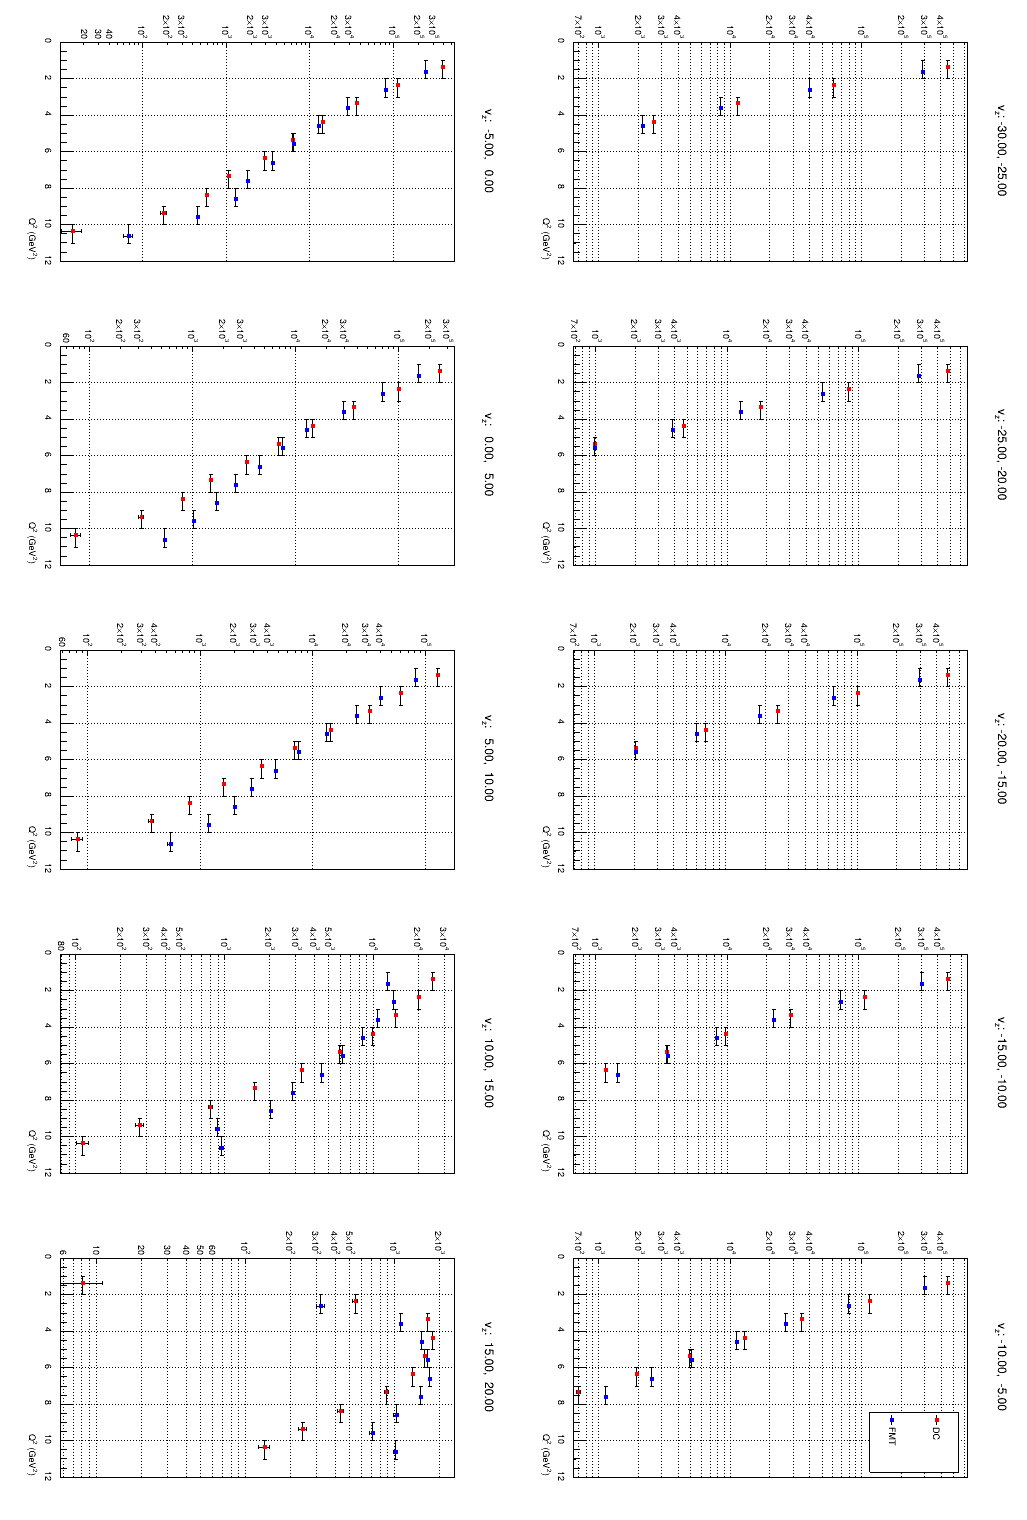
\includegraphics[width=\textwidth]{31q2_vz.png}
        \caption[Acceptance-corrected $Q^2$ separated in $v_z$ bins]
        {Acceptance-corrected $Q^2$ detected by DC and FMT, separated in $v_z$ bins.
        Run 12016.
        The bin markers are slightly shifted in $x$ to improve legibility.}
        \floatfoot{Source: Own elaboration, using the \href{https://github.com/bleaktwig/clas12-rge-analysis}{clas12-rge-analysis} software.}
        \label{fig::14.31::q2_vz}
    \end{figure}

    % nu.
    \begin{figure}
        \centering
        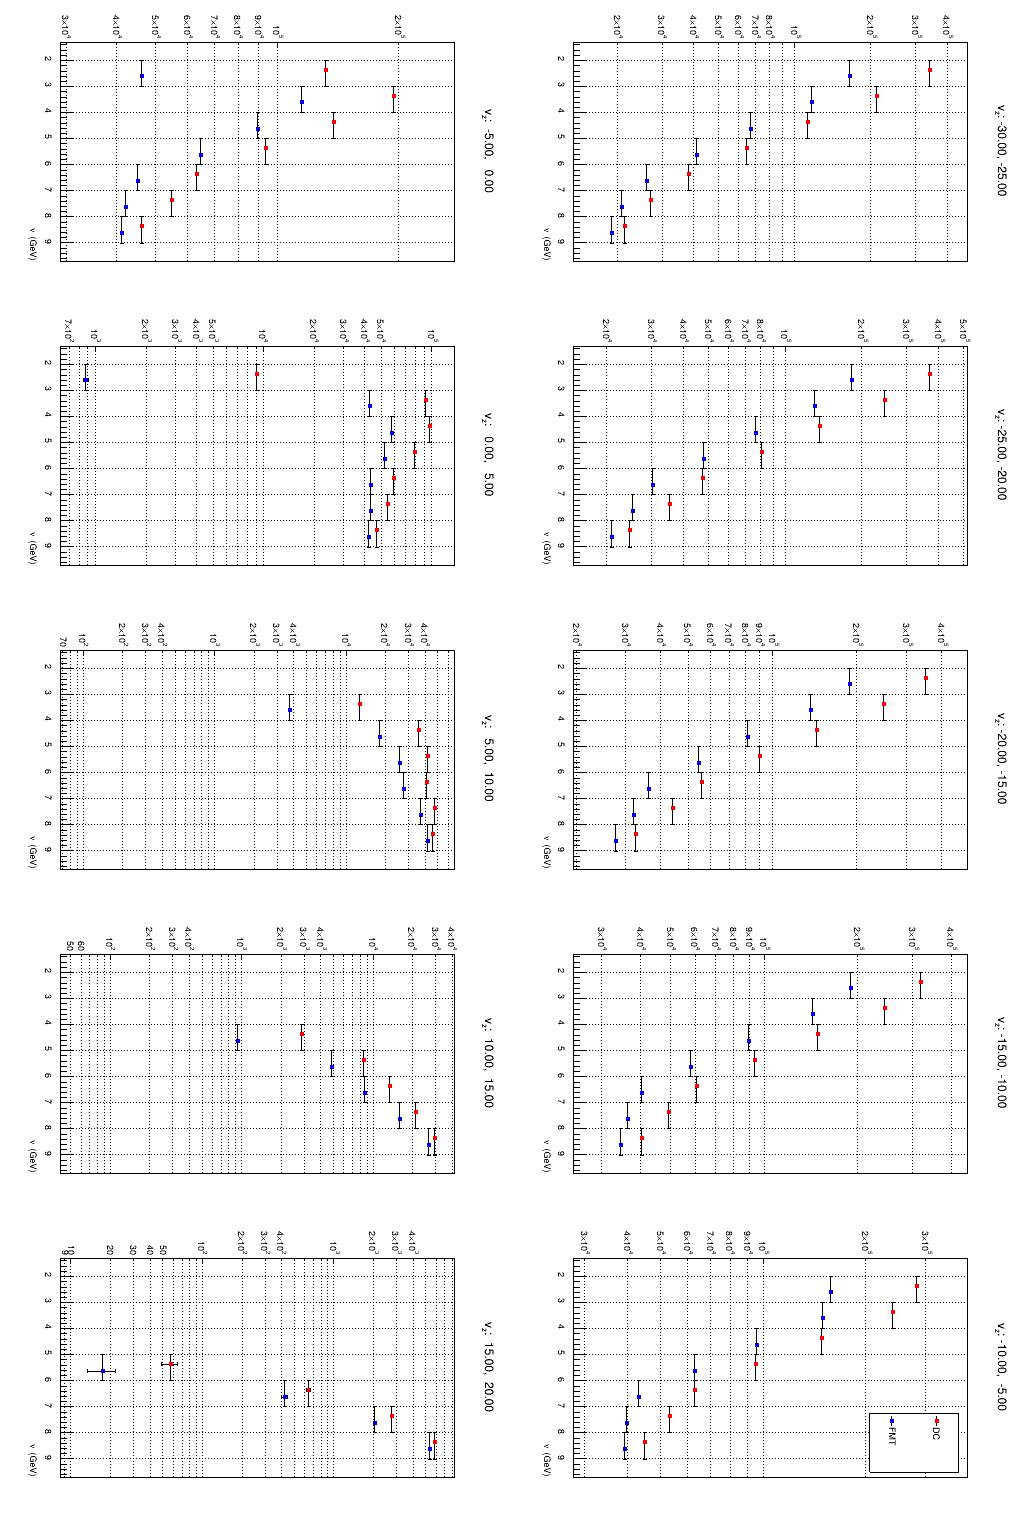
\includegraphics[width=\textwidth]{31nu_vz.png}
        \caption[Acceptance-corrected $\nu$ separated in $v_z$ bins]
        {Acceptance-corrected $\nu$ detected by DC and FMT, separated in $v_z$ bins.
        Run 12016.
        The bin markers are slightly shifted in $x$ to improve legibility.}
        \floatfoot{Source: Own elaboration, using the \href{https://github.com/bleaktwig/clas12-rge-analysis}{clas12-rge-analysis} software.}
        \label{fig::14.31::nu_vz}
    \end{figure}

    % zh.
    \begin{figure}
        \centering
        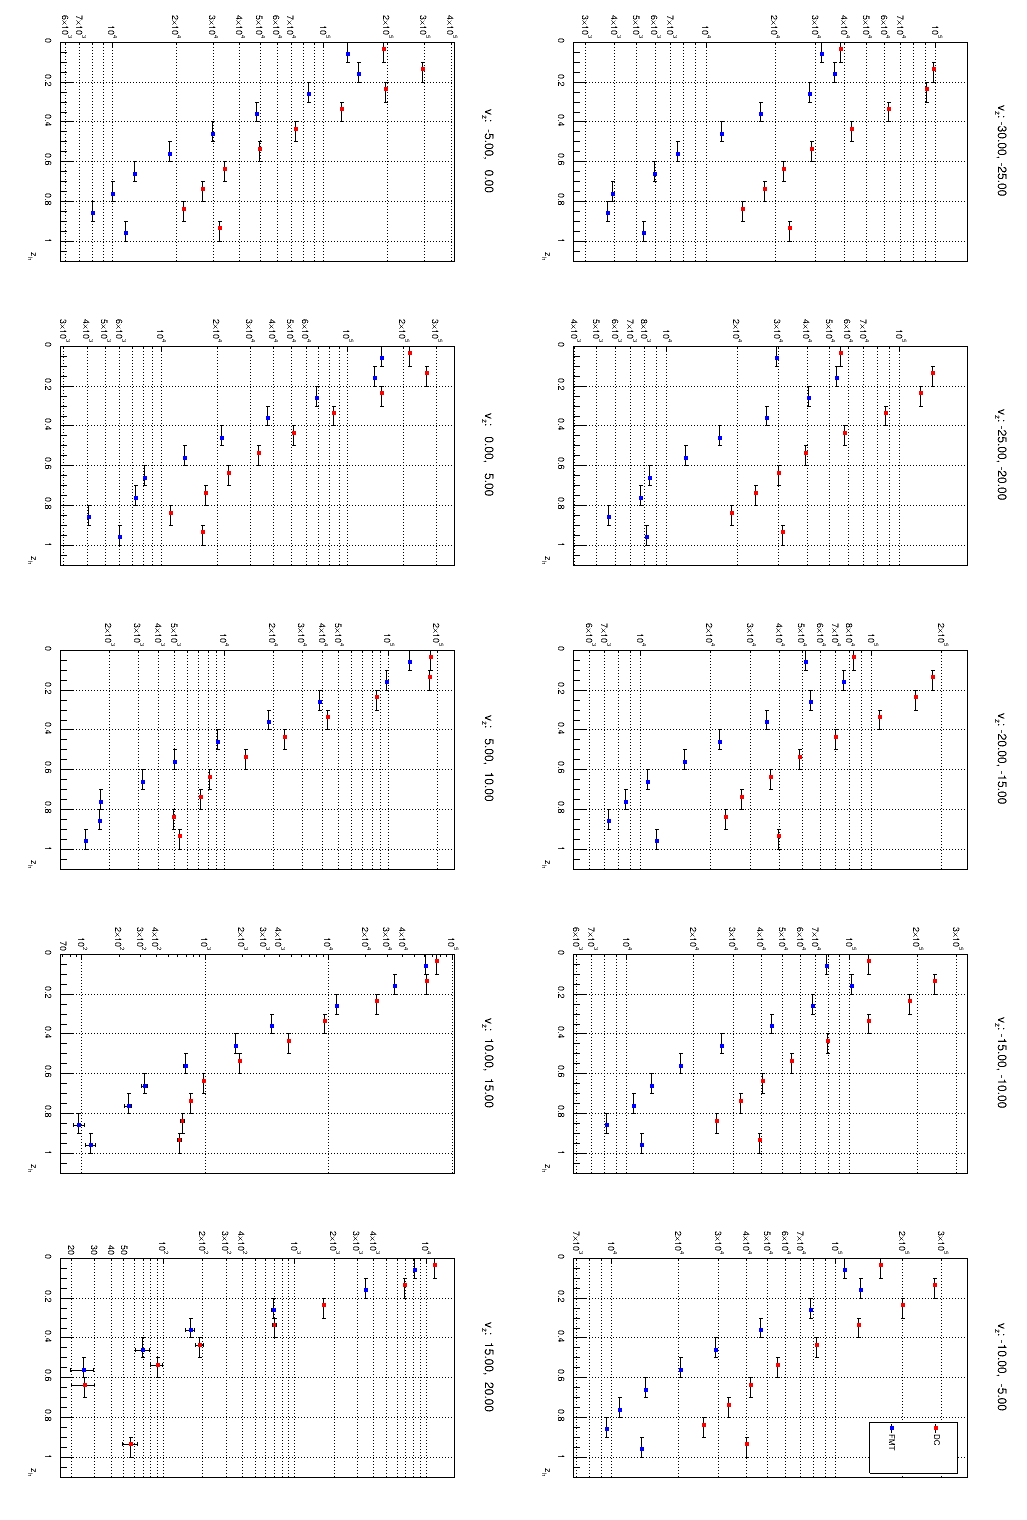
\includegraphics[width=\textwidth]{31zh_vz_211.png}
        \caption[Acceptance-corrected $z_h$ for $e^-\pi^+$ separated in $v_z$ bins]
        {Acceptance-corrected $z_h$ for $e^-\pi^+$ detected by DC and FMT, separated in $v_z$ bins.
        Run 12016.
        The bin markers are slightly shifted in $x$ to improve legibility.}
        \floatfoot{Source: Own elaboration, using the \href{https://github.com/bleaktwig/clas12-rge-analysis}{clas12-rge-analysis} software.}
        \label{fig::14.31::zh_211_vz}
    \end{figure}

    \begin{figure}
        \centering
        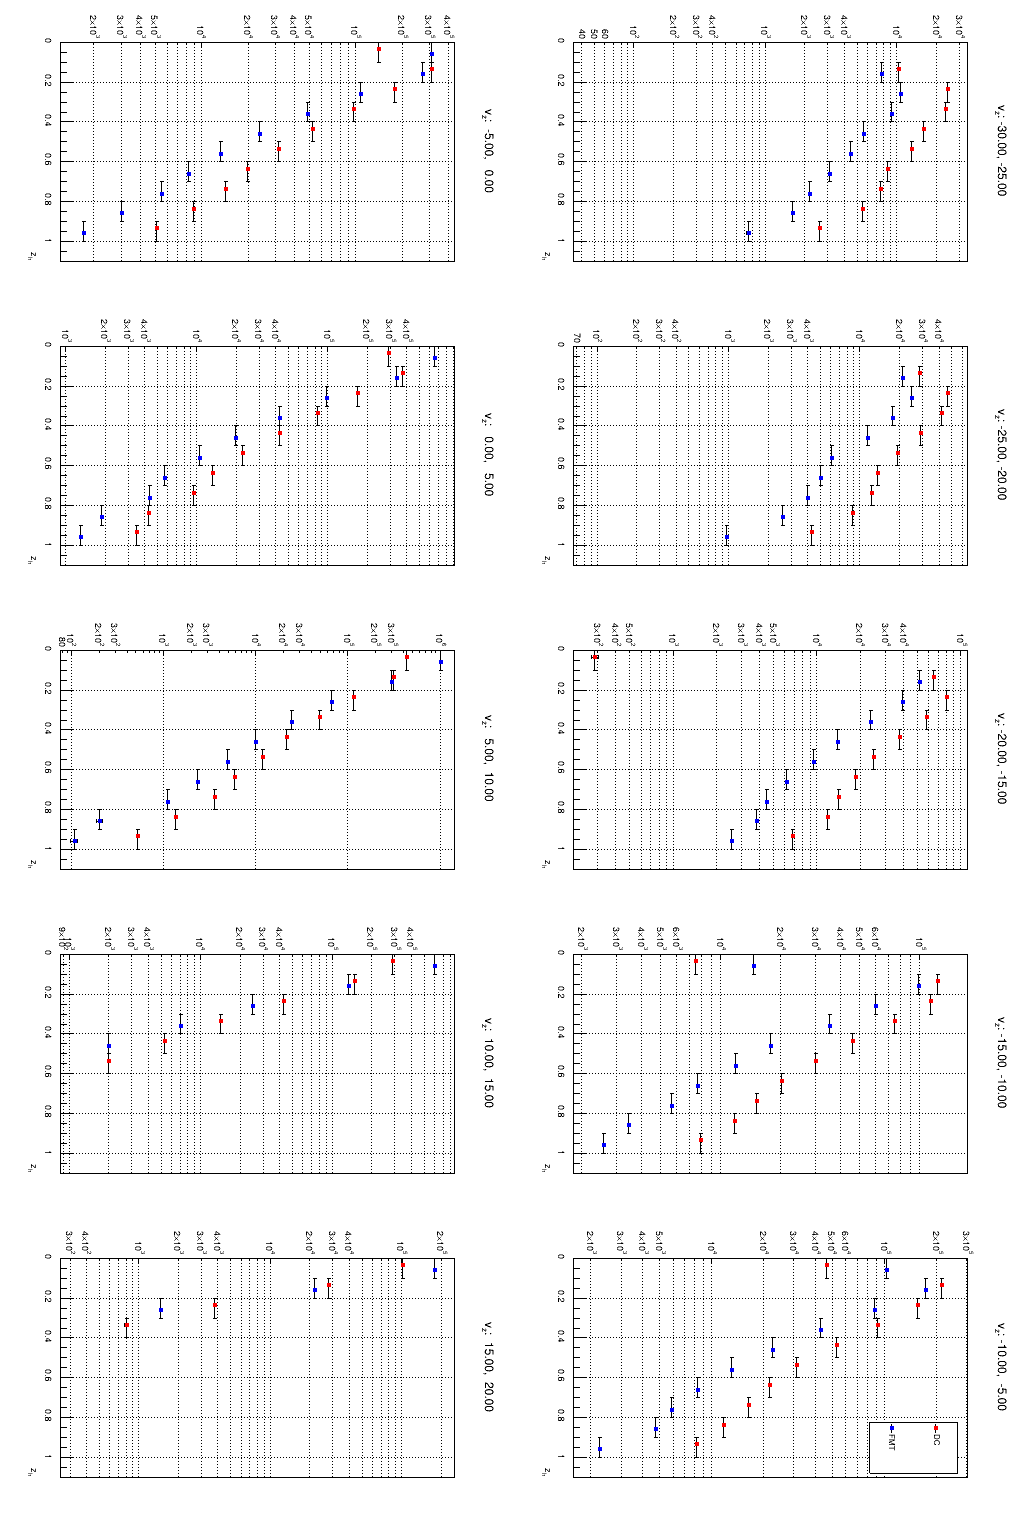
\includegraphics[width=\textwidth]{31zh_vz_-211.png}
        \caption[Acceptance-corrected $z_h$ for $e^-\pi^-$ separated in $v_z$ bins]
        {Acceptance-corrected $z_h$ for $e^-\pi^-$ detected by DC and FMT, separated in $v_z$ bins.
        Run 12016.
        The bin markers are slightly shifted in $x$ to improve legibility.}
        \floatfoot{Source: Own elaboration, using the \href{https://github.com/bleaktwig/clas12-rge-analysis}{clas12-rge-analysis} software.}
        \label{fig::14.31::zh_-211_vz}
    \end{figure}

    % pt2.
    \begin{figure}
        \centering
        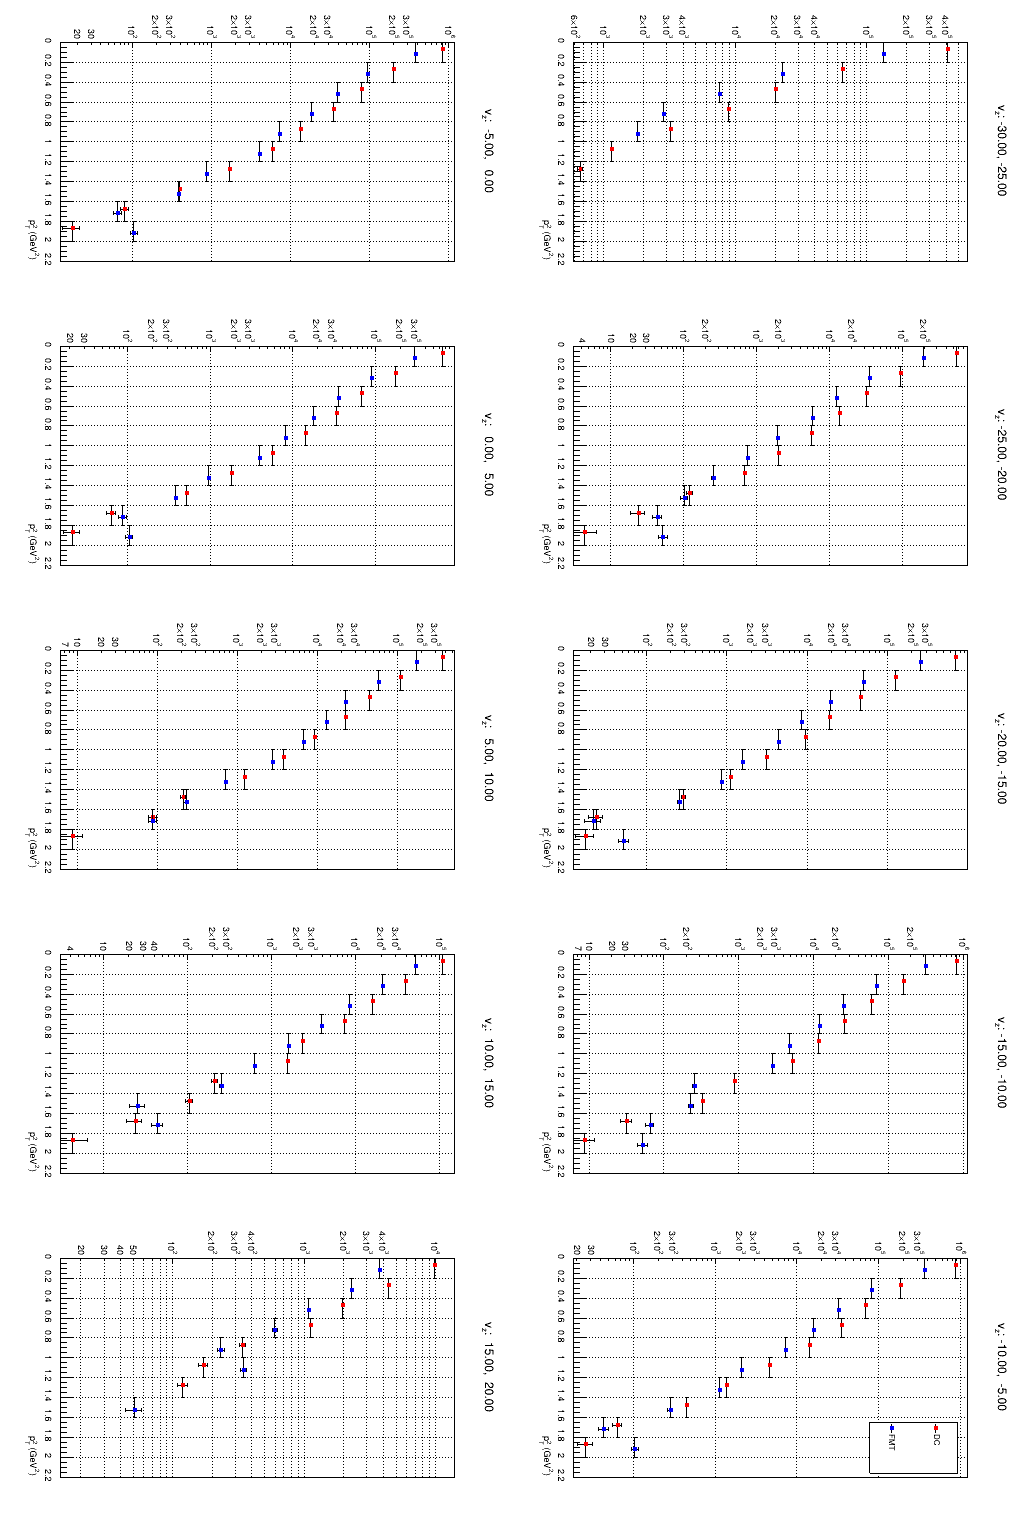
\includegraphics[width=\textwidth]{31pt2_vz_211.png}
        \caption[Acceptance-corrected $p_T^2$ for $e^-\pi^+$ separated in $v_z$ bins]
        {Acceptance-corrected $p_T^2$ for $e^-\pi^+$ detected by DC and FMT, separated in $v_z$ bins.
        Run 12016.
        The bin markers are slightly shifted in $x$ to improve legibility.}
        \floatfoot{Source: Own elaboration, using the \href{https://github.com/bleaktwig/clas12-rge-analysis}{clas12-rge-analysis} software.}
        \label{fig::14.31::pt2_211_vz}
    \end{figure}

    \begin{figure}
        \centering
        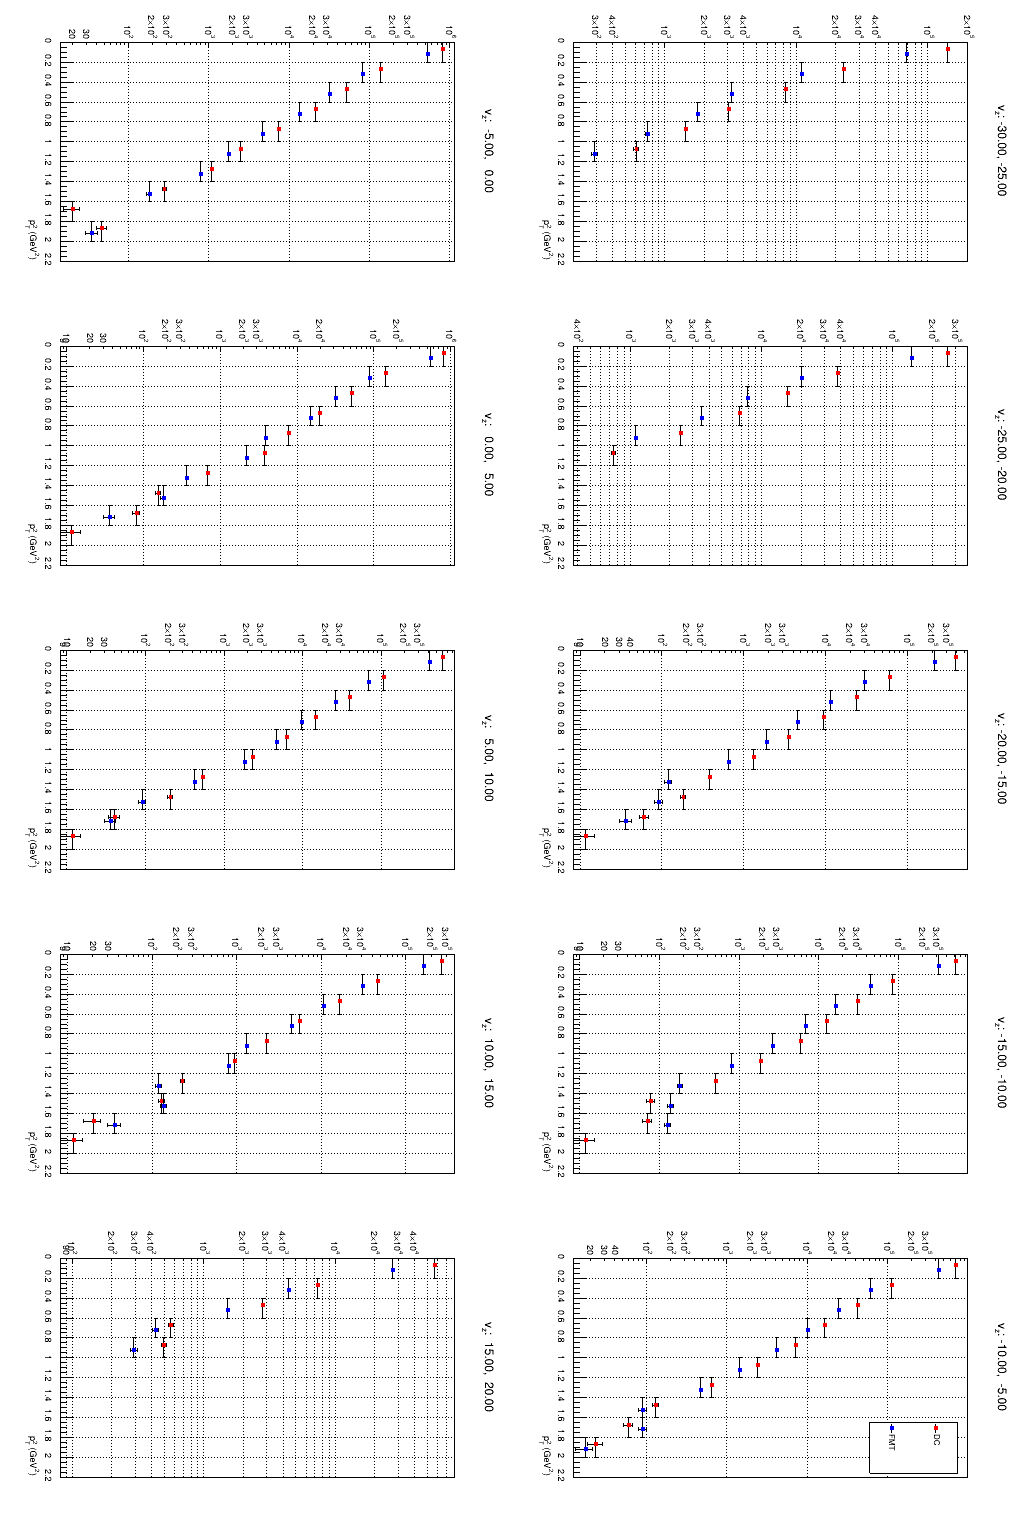
\includegraphics[width=\textwidth]{31pt2_vz_-211.png}
        \caption[Acceptance-corrected $p_T^2$ for $e^-\pi^-$ separated in $v_z$ bins]
        {Acceptance-corrected $p_T^2$ for $e^-\pi^-$ detected by DC and FMT, separated in $v_z$ bins.
        Run 12016.
        The bin markers are slightly shifted in $x$ to improve legibility.}
        \floatfoot{Source: Own elaboration, using the \href{https://github.com/bleaktwig/clas12-rge-analysis}{clas12-rge-analysis} software.}
        \label{fig::14.31::pt2_-211_vz}
    \end{figure}

    % phipq.
    \begin{figure}
        \centering
        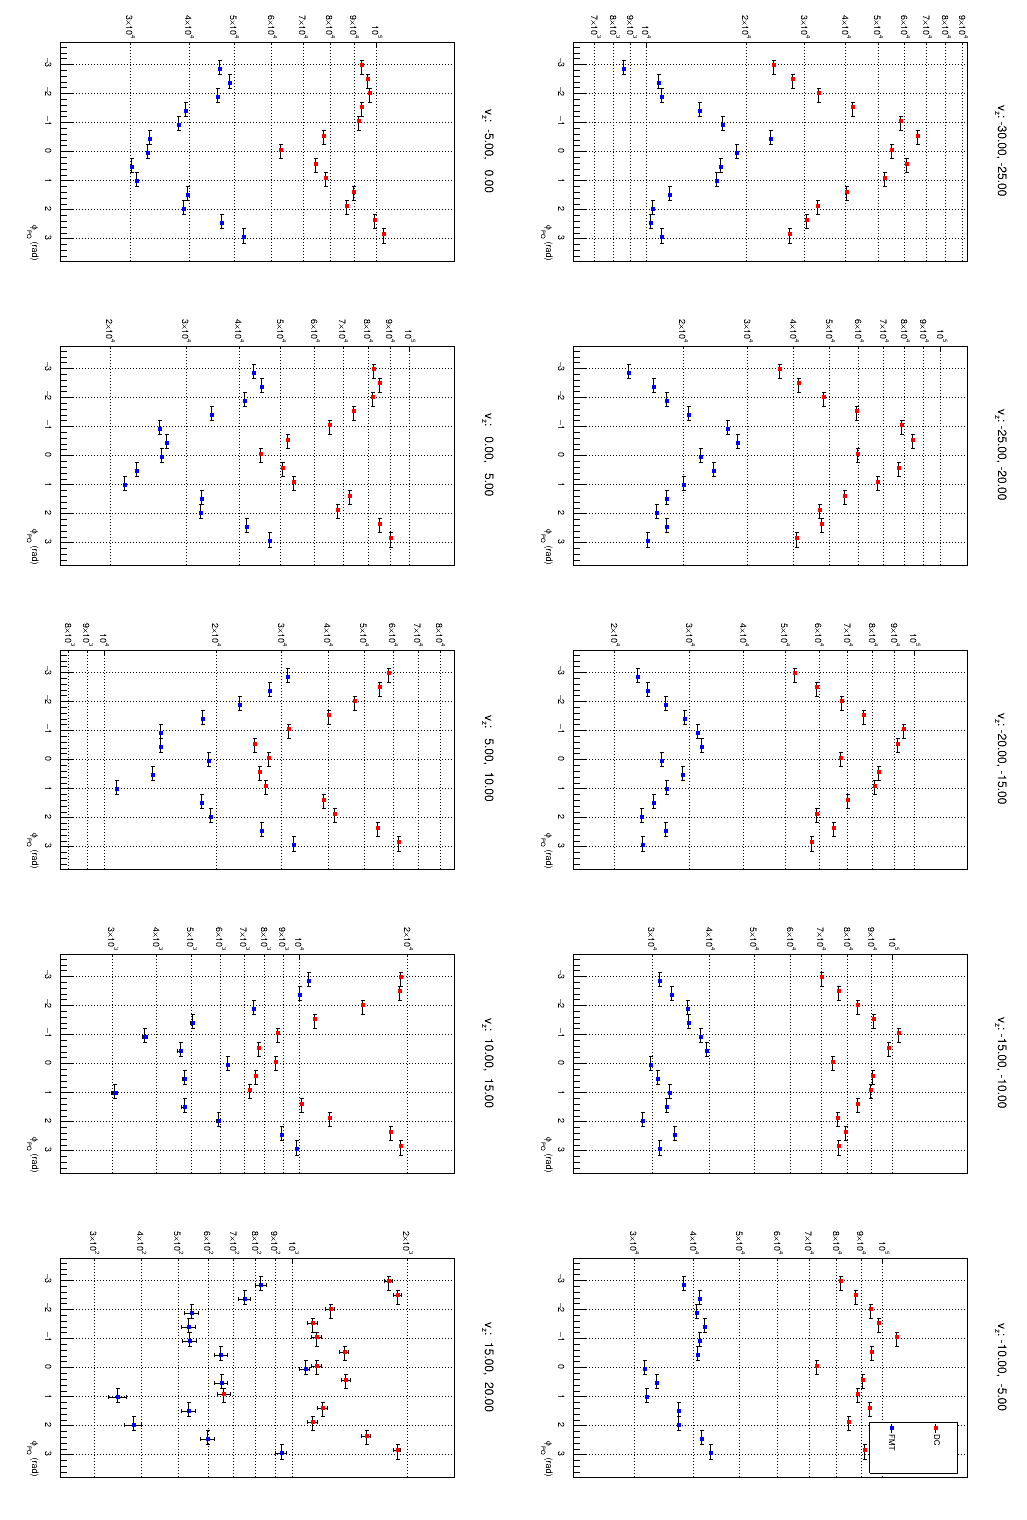
\includegraphics[width=\textwidth]{31phipq_vz_211.png}
        \caption[Acceptance-corrected $\phi_{PQ}$ for $e^-\pi^+$ separated in $v_z$ bins]
        {Acceptance-corrected $\phi_{PQ}$ for $e^-\pi^+$ detected by DC and FMT, separated in $v_z$ bins.
        Run 12016.
        The bin markers are slightly shifted in $x$ to improve legibility.}
        \floatfoot{Source: Own elaboration, using the \href{https://github.com/bleaktwig/clas12-rge-analysis}{clas12-rge-analysis} software.}
        \label{fig::14.31::phipq_211_vz}
    \end{figure}

    \begin{figure}
        \centering
        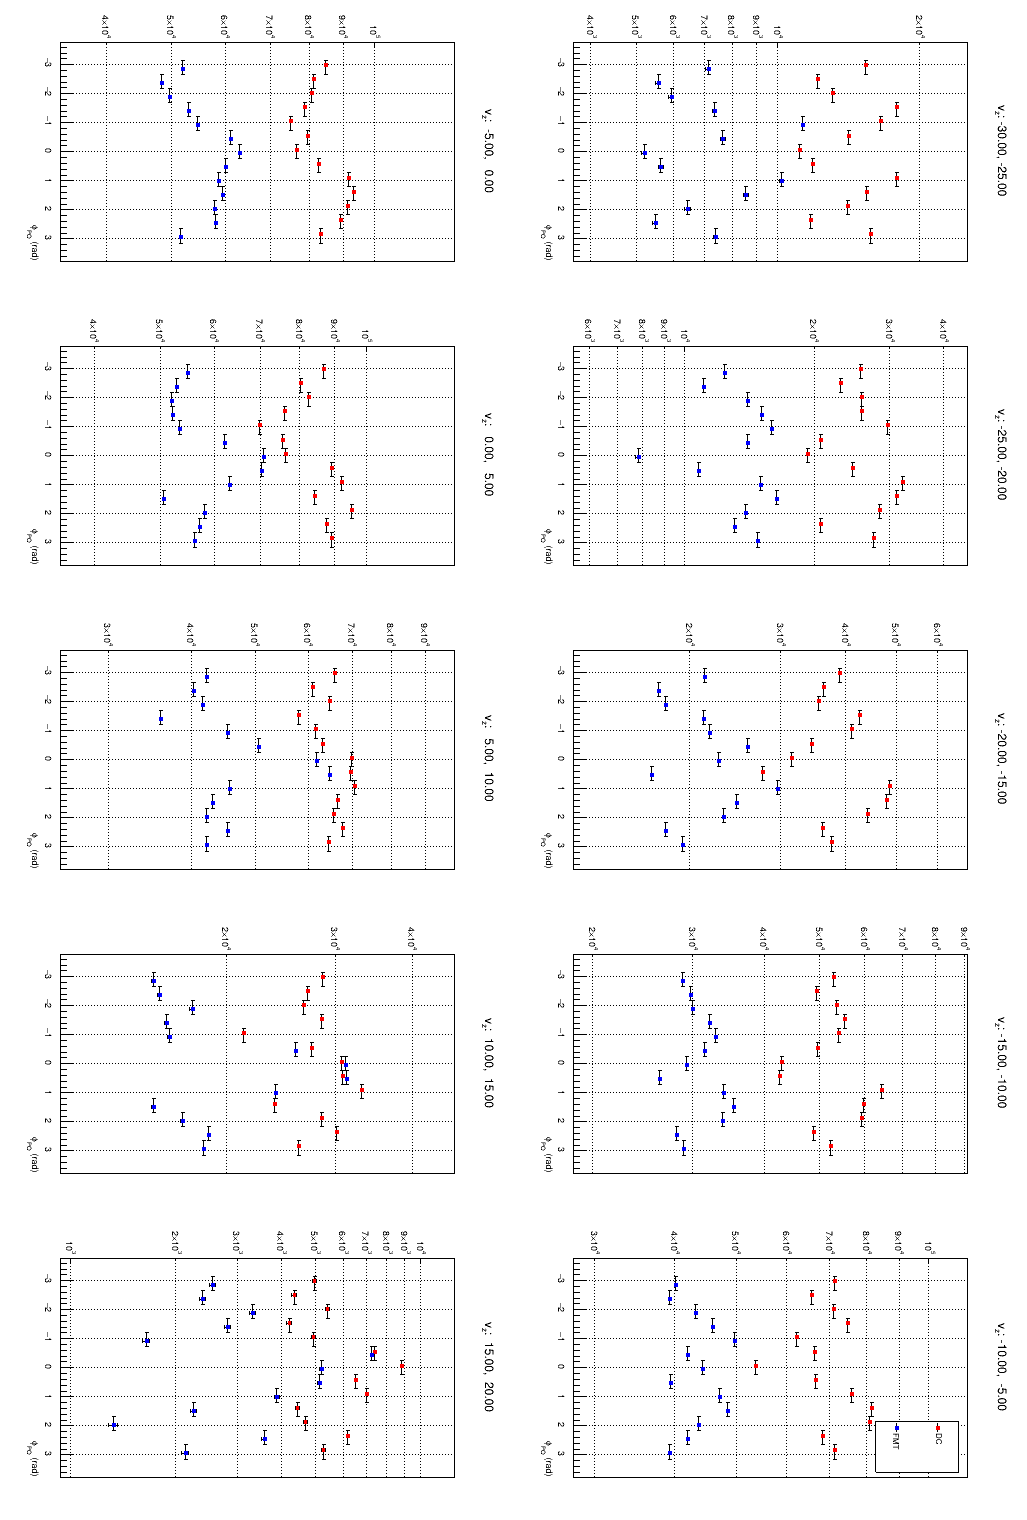
\includegraphics[width=\textwidth]{31phipq_vz_-211.png}
        \caption[Acceptance-corrected $\phi_{PQ}$ for $e^-\pi^-$ separated in $v_z$ bins]
        {Acceptance-corrected $\phi_{PQ}$ for $e^-\pi^-$ detected by DC and FMT, separated in $v_z$ bins.
        Run 12016.
        The bin markers are slightly shifted in $x$ to improve legibility.}
        \floatfoot{Source: Own elaboration, using the \href{https://github.com/bleaktwig/clas12-rge-analysis}{clas12-rge-analysis} software.}
        \label{fig::14.31::phipq_-211_vz}
    \end{figure}

    % statistics.
    \begin{figure}
        \centering
        % e-.
        \begin{subfigure}[b]{\textwidth}
            \centering
            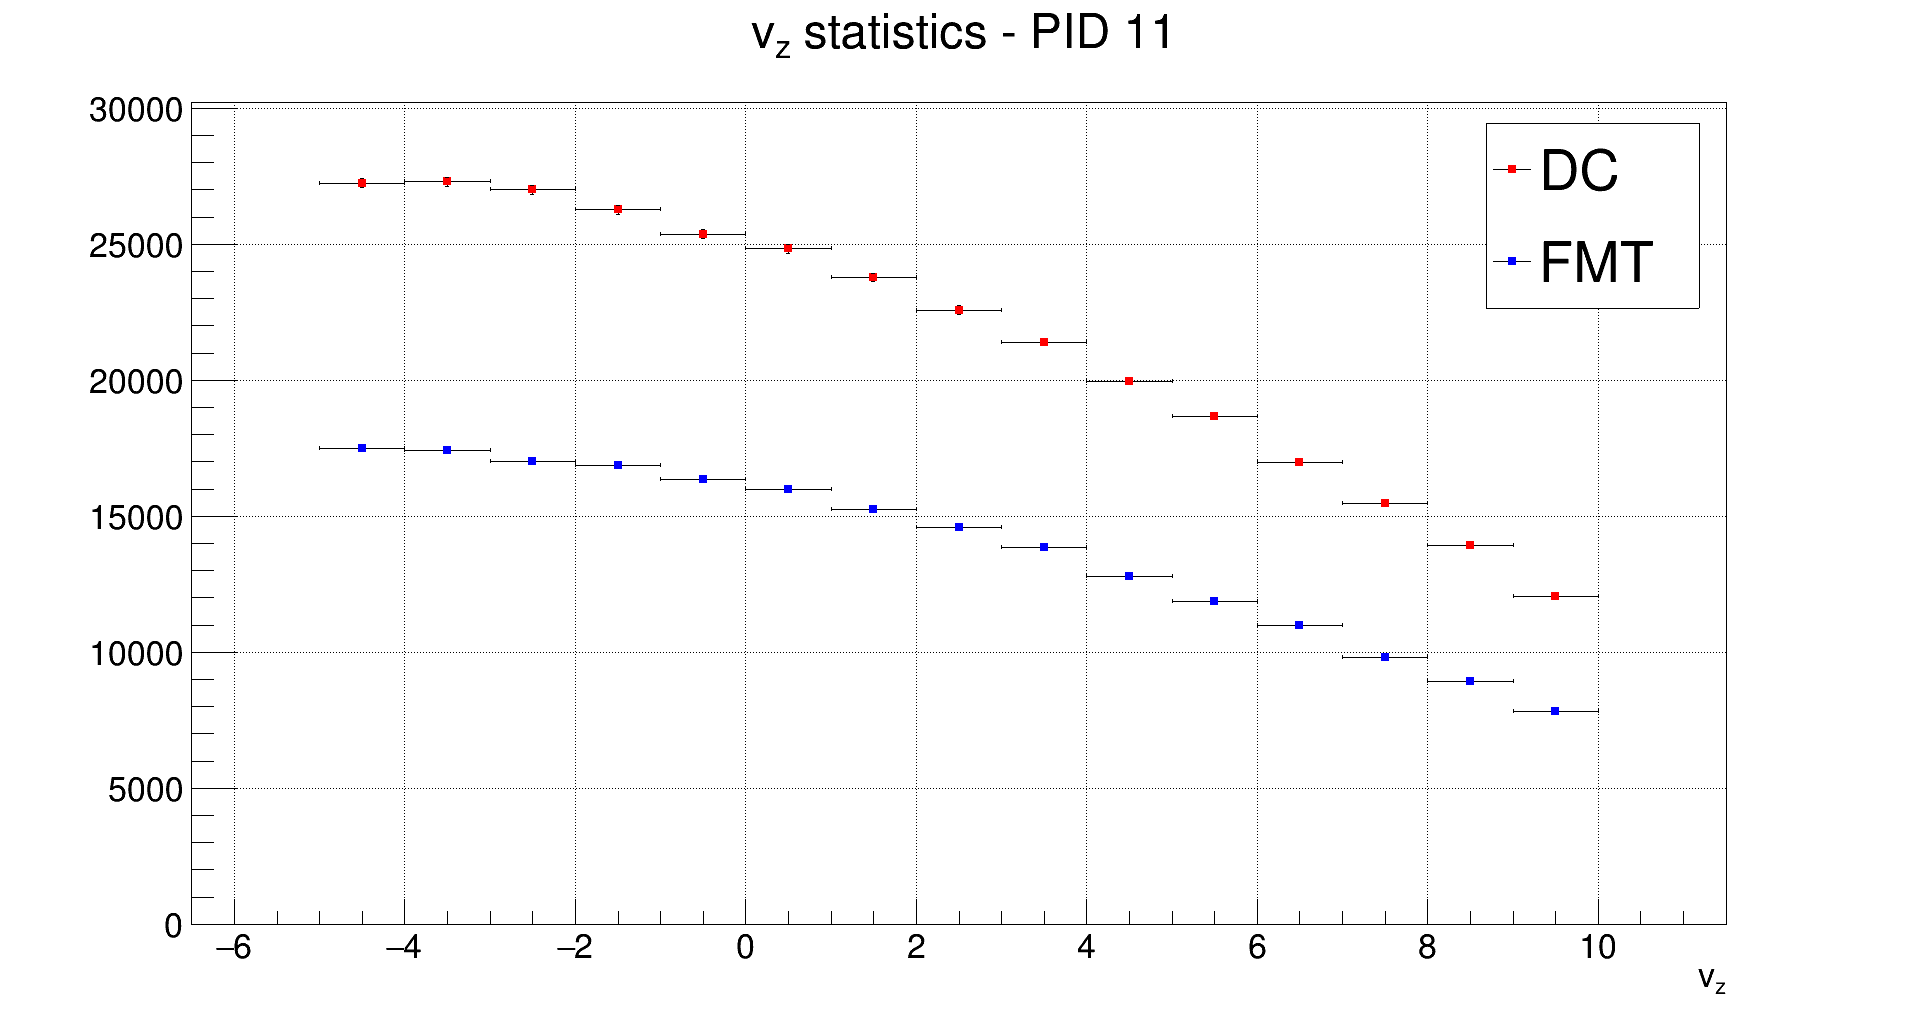
\includegraphics[width=\textwidth]{32statistics_11.png}
            \caption{$e^-$ statistics.}
            \label{fig::14.32::statistics_11}
        \end{subfigure}
        \centering
        % e-pi+.
        \begin{subfigure}[b]{0.49\textwidth}
            \centering
            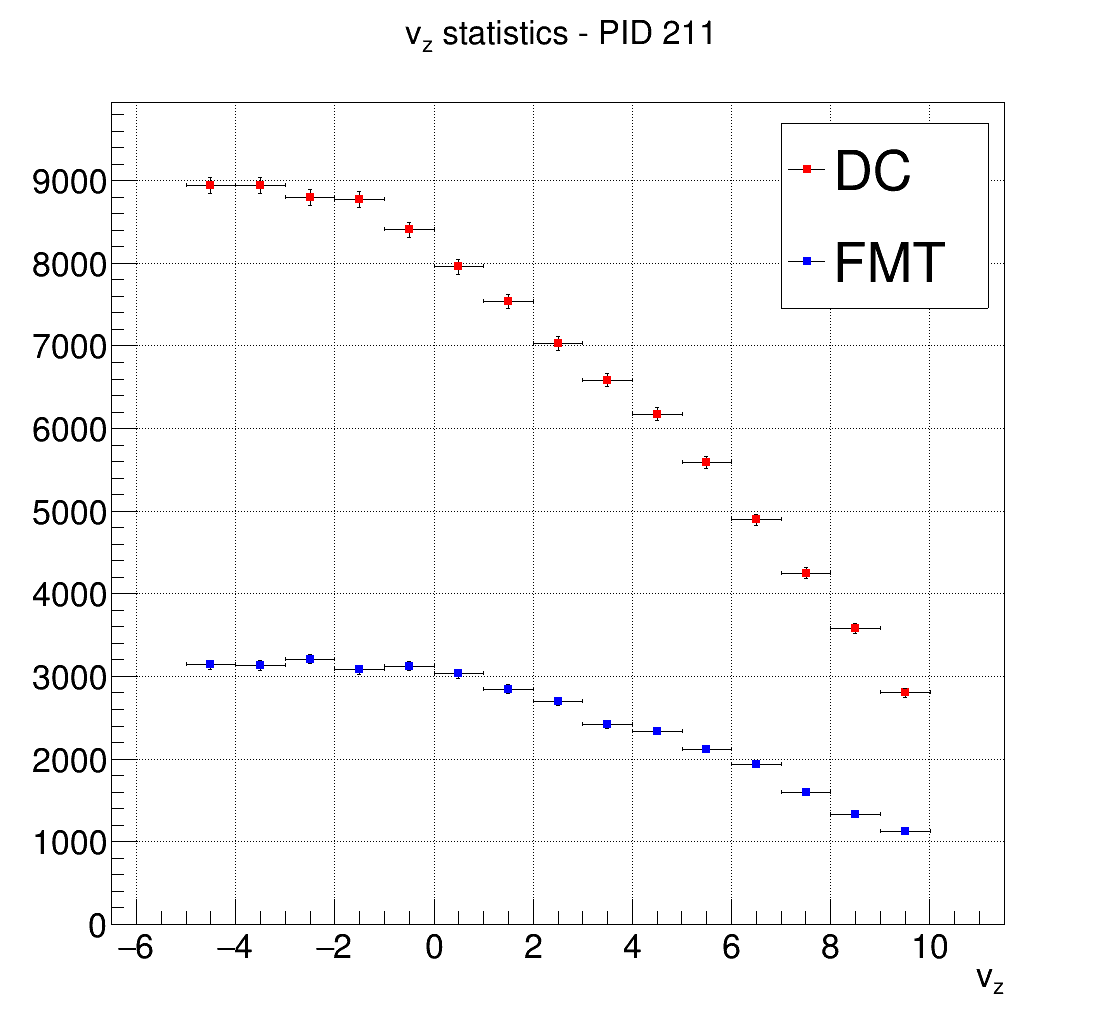
\includegraphics[width=\textwidth]{32statistics_211.png}
            \caption{$e^-\pi^+$ statistics.}
            \label{fig::14.32::statistics_211}
        \end{subfigure}
        \hfill
        % e-pi-.
        \begin{subfigure}[b]{0.49\textwidth}
            \centering
            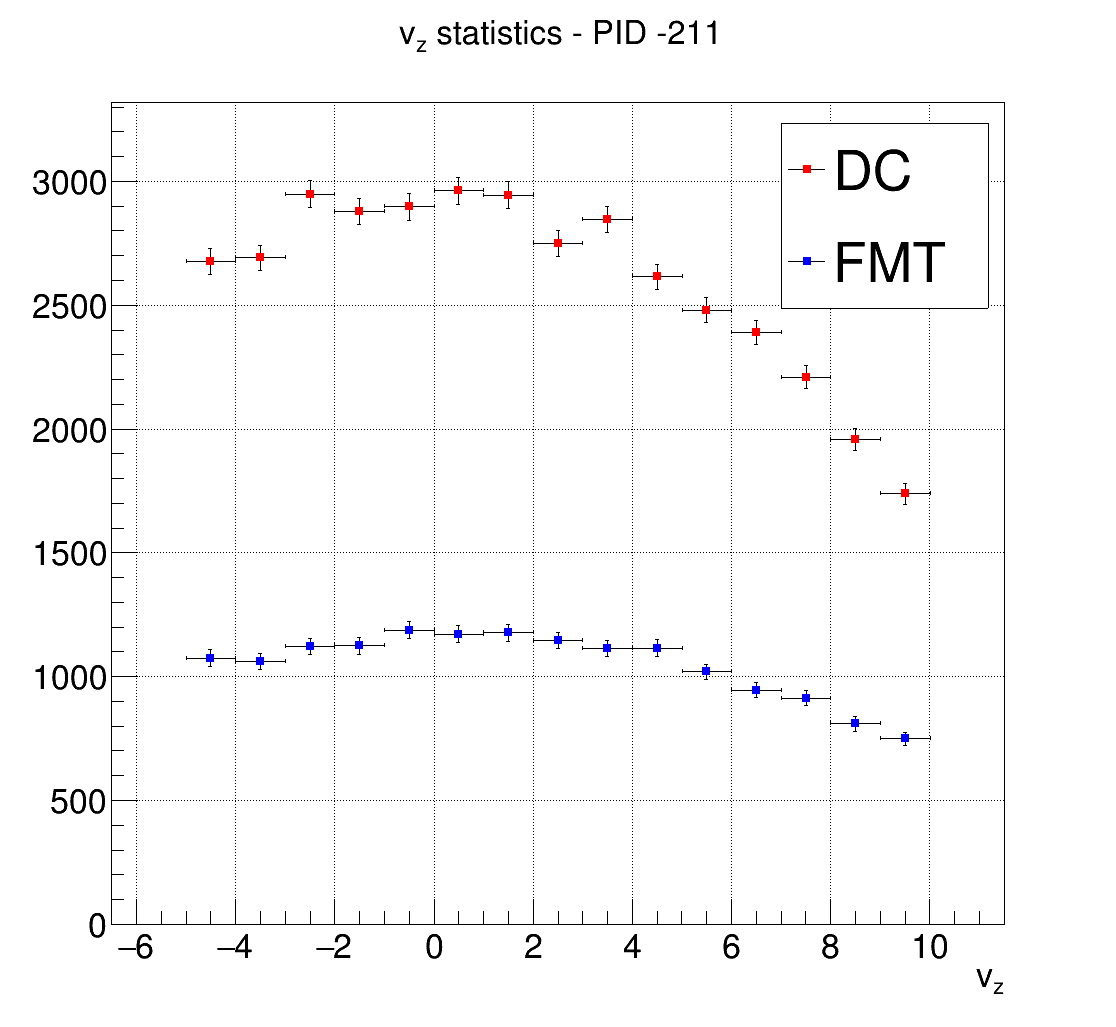
\includegraphics[width=\textwidth]{32statistics_-211.png}
            \caption{$e^-\pi^-$ statistics.}
            \label{fig::14.32::statistics_-211}
        \end{subfigure}
        \caption[Statistics for $e^-$, $e^-\pi^+$, and $e^-\pi^-$ against $v_z$]
        {$e^-$, $e^-\pi^+$, and $e^-\pi^-$ statistics against $v_z$ for run 12016.
        No acceptance correction was applied to these results.}
        \floatfoot{Source: Own elaboration, using the \href{https://github.com/bleaktwig/clas12-rge-analysis}{clas12-rge-analysis} software.}
        \label{fig::14.32::statistics}
    \end{figure}
